%%=============================================================================
%% LaTeX sjabloon voor bachelorproef, HoGent Bedrijf en Organisatie
%% Opleiding Toegepaste Informatica
%%=============================================================================

\documentclass[fleqn,a4paper,12pt]{book}

%%=============================================================================
%% LaTeX sjabloon voor de bachelorproef, HoGent Bedrijf en Organisatie
%% Opleiding toegepaste informatica
%%
%% Structuur en algemene vormgeving. Meestal hoef je hier niets te wijzigen.
%%
%% Vormgeving gebaseerd op "The Legrand Orange Book", version 2.0 (9/2/15)
%% door Mathias Legrand (legrand.mathias@gmail.com) met aanpassingen door
%% Vel (vel@latextemplates.com). Het oorspronkelijke template is te vinden op
%% http://www.LaTeXTemplates.com
%%
%% Aanpassingen voor HoGent toegepaste informatica: 
%%   Bert Van Vreckem <bert.vanvreckem@hogent.be>
%% Licentie: 
%%   CC BY-NC-SA 3.0 (http://creativecommons.org/licenses/by-nc-sa/3.0/)
%%=============================================================================

%%-----------------------------------------------------------------------------
%% Packages
%%-----------------------------------------------------------------------------

\usepackage[top=3cm,bottom=3cm,left=3cm,right=3cm,headsep=10pt,a4paper]{geometry} % Page margins
\usepackage[utf8]{inputenc}  % Accenten gebruiken in tekst (vb. é ipv \'e)
\usepackage{amsfonts}        % AMS math packages: extra wiskundige
\usepackage{amsmath}         %   symbolen (o.a. getallen-
\usepackage{amssymb}         %   verzamelingen N, R, Z, Q, etc.)
\usepackage[english,dutch]{babel}    % Taalinstellingen: woordsplitsingen,
                             %  commando's voor speciale karakters
                             %  ("dutch" voor NL)
\usepackage{iflang}
\usepackage{eurosym}         % Euro-symbool €
\usepackage{geometry}
\usepackage{graphicx}        % Invoegen van tekeningen
\graphicspath{{img/}}       % Specifies the directory where pictures are stored
\usepackage{tikz}            % Required for drawing custom shapes
\usepackage[pdftex,bookmarks=true]{hyperref}
                             % PDF krijgt klikbare links & verwijzingen,
                             %  inhoudstafel
\usepackage{enumitem}        % Customize lists
\setlist{nolistsep}         % Reduce spacing between list items
\usepackage{listings}        % Broncode mooi opmaken
\usepackage{multirow}        % Tekst over verschillende cellen in tabellen
\usepackage{rotating}        % Tabellen en figuren roteren

\usepackage{booktabs}        % Required for nicer horizontal rules in tables

\usepackage{xcolor}          % Required for specifying colors by name
\definecolor{maincolor}{RGB}{0,147,208} % Define the main color used for 
                             % highlighting throughout the book
                             % 0, 147, 208 = officiële kleur HoGent FBO

% Paragraph style: no indent, add space between paragraphs
\setlength{\parindent}{0em}
\setlength{\parskip}{1em}

\usepackage{etoolbox}
\usepackage{titling} % Macros for title, author, etc
\usepackage{glossaries}
\makeglossaries

%----------------------------------------------------------------------------------------
%	FONTS
%----------------------------------------------------------------------------------------

\usepackage{avant} % Use the Avantgarde font for headings
%\usepackage{times} % Use the Times font for headings
\usepackage{mathptmx} % Use the Adobe Times Roman as the default text font together with math symbols from the Sym­bol, Chancery and Com­puter Modern fonts

\usepackage{microtype} % Slightly tweak font spacing for aesthetics
\usepackage[utf8]{inputenc} % Required for including letters with accents
\usepackage[T1]{fontenc} % Use 8-bit encoding that has 256 glyphs

%------------------------------------------------------------------------------
%	TITLE PAGE
%------------------------------------------------------------------------------

\newcommand{\inserttitlepage}{%
\begin{titlepage}
  \newgeometry{top=2cm,bottom=1.5cm,left=1.5cm,right=1.5cm}
  \begin{center}

    \begingroup
    \rmfamily
    \includegraphics[width=2.5cm]{img/HG-beeldmerk-woordmerk}\\[.5cm]
    Faculteit Bedrijf en Organisatie\\[3cm]
    \titel
    \vfill
    \student\\[3.5cm]
    Scriptie voorgedragen tot het bekomen van de graad van\\professionele bachelor in de toegepaste informatica\\[2cm]
    Promotor:\\
    \promotor\\
    \ifdefempty{\copromotor}{\vspace{2.5cm}}{Co-promotor:\\\copromotor\\[2.5cm]}
    Instelling: \instelling\\[.5cm]
    Academiejaar: \academiejaar\\[.5cm]
    \ifcase \examenperiode \or Eerste \or Tweede \else Derde \fi examenperiode
    \endgroup

  \end{center}
  \restoregeometry
\end{titlepage}
  \emptypage
\begin{titlepage}
  \newgeometry{top=5.35cm,bottom=1.5cm,left=1.5cm,right=1.5cm}
  \begin{center}

    \begingroup
    \rmfamily
    \IfLanguageName{dutch}{Faculteit Bedrijf en Organisatie}{Faculty of Business and Information Management}\\[3cm]
    \titel
    \vfill
    \student\\[3.5cm]
    \IfLanguageName{dutch}{Scriptie voorgedragen tot het bekomen van de graad van\\professionele bachelor in de toegepaste informatica}{Thesis submitted in partial fulfilment of the requirements for the degree of\\professional bachelor of applied computer science}\\[2cm]
    Promotor:\\
    \promotor\\
    \ifdefempty{\copromotor}{\vspace{2.5cm}}{Co-promotor:\\\copromotor\\[2.5cm]}
    \IfLanguageName{dutch}{Instelling}{Institution}: \instelling\\[.5cm]
    \IfLanguageName{dutch}{Academiejaar}{Academic year}: \academiejaar\\[.5cm]
    \IfLanguageName{dutch}{%
    \ifcase \examenperiode \or Eerste \or Tweede \else Derde \fi examenperiode}{%
    \ifcase \examenperiode \or First \or Second \else Third \fi examination period}
    \endgroup

  \end{center}
  \restoregeometry
\end{titlepage}
}

%----------------------------------------------------------------------------------------
%	BIBLIOGRAPHY AND INDEX
%----------------------------------------------------------------------------------------

\usepackage[style=apa,backend=biber]{biblatex}
\usepackage{csquotes}
\DeclareLanguageMapping{dutch}{dutch-apa}
\addbibresource{bachproef-tin.bib} % BibTeX bibliography file
\addbibresource{../voorstel/voorstel.bib}
\defbibheading{bibempty}{}

\usepackage{calc} % For simpler calculation - used for spacing the index letter headings correctly
\usepackage{makeidx} % Required to make an index
\makeindex % Tells LaTeX to create the files required for indexing

%----------------------------------------------------------------------------------------
%	MAIN TABLE OF CONTENTS
%----------------------------------------------------------------------------------------

\usepackage{titletoc} % Required for manipulating the table of contents

\contentsmargin{0cm} % Removes the default margin

% Part text styling
\titlecontents{part}[0cm]
{\addvspace{20pt}\centering\large\bfseries}
{}
{}
{}

% Chapter text styling
\titlecontents{chapter}[1.25cm] % Indentation
{\addvspace{12pt}\large\sffamily\bfseries} % Spacing and font options for chapters
{\color{maincolor!60}\contentslabel[\Large\thecontentslabel]{1.25cm}\color{maincolor}} % Chapter number
{\color{maincolor}}
{\color{maincolor!60}\normalsize\;\titlerule*[.5pc]{.}\;\thecontentspage} % Page number

% Section text styling
\titlecontents{section}[1.25cm] % Indentation
{\addvspace{3pt}\sffamily\bfseries} % Spacing and font options for sections
{\contentslabel[\thecontentslabel]{1.25cm}} % Section number
{}
{\hfill\color{black}\thecontentspage} % Page number
[]

% Subsection text styling
\titlecontents{subsection}[1.25cm] % Indentation
{\addvspace{1pt}\sffamily\small} % Spacing and font options for subsections
{\contentslabel[\thecontentslabel]{1.25cm}} % Subsection number
{}
{\ \titlerule*[.5pc]{.}\;\thecontentspage} % Page number
[]

% List of figures
\titlecontents{figure}[0em]
{\addvspace{-5pt}\sffamily}
{\thecontentslabel\hspace*{1em}}
{}
{\ \titlerule*[.5pc]{.}\;\thecontentspage}
[]

% List of tables
\titlecontents{table}[0em]
{\addvspace{-5pt}\sffamily}
{\thecontentslabel\hspace*{1em}}
{}
{\ \titlerule*[.5pc]{.}\;\thecontentspage}
[]

%----------------------------------------------------------------------------------------
%	MINI TABLE OF CONTENTS IN PART HEADS
%----------------------------------------------------------------------------------------

% Chapter text styling
\titlecontents{lchapter}[0em] % Indenting
{\addvspace{15pt}\large\sffamily\bfseries} % Spacing and font options for chapters
{\color{maincolor}\contentslabel[\Large\thecontentslabel]{1.25cm}\color{maincolor}} % Chapter number
{}
{\color{maincolor}\normalsize\sffamily\bfseries\;\titlerule*[.5pc]{.}\;\thecontentspage} % Page number

% Section text styling
\titlecontents{lsection}[0em] % Indenting
{\sffamily\small} % Spacing and font options for sections
{\contentslabel[\thecontentslabel]{1.25cm}} % Section number
{}
{}

% Subsection text styling
\titlecontents{lsubsection}[.5em] % Indentation
{\normalfont\footnotesize\sffamily} % Font settings
{}
{}
{}

%----------------------------------------------------------------------------------------
%	PAGE HEADERS
%----------------------------------------------------------------------------------------

\usepackage{fancyhdr} % Required for header and footer configuration

\pagestyle{fancy}
\renewcommand{\chaptermark}[1]{\markboth{\sffamily\normalsize\bfseries\chaptername\ \thechapter.\ #1}{}} % Chapter text font settings
\renewcommand{\sectionmark}[1]{\markright{\sffamily\normalsize\thesection\hspace{5pt}#1}{}} % Section text font settings
\fancyhf{} \fancyhead[LE,RO]{\sffamily\normalsize\thepage} % Font setting for the page number in the header
\fancyhead[LO]{\rightmark} % Print the nearest section name on the left side of odd pages
\fancyhead[RE]{\leftmark} % Print the current chapter name on the right side of even pages
\renewcommand{\headrulewidth}{0.5pt} % Width of the rule under the header
\addtolength{\headheight}{2.5pt} % Increase the spacing around the header slightly
\renewcommand{\footrulewidth}{0pt} % Removes the rule in the footer
\fancypagestyle{plain}{\fancyhead{}\renewcommand{\headrulewidth}{0pt}} % Style for when a plain pagestyle is specified

% Removes the header from odd empty pages at the end of chapters
\makeatletter
\renewcommand{\cleardoublepage}{
\clearpage\ifodd\c@page\else
\hbox{}
\vspace*{\fill}
\thispagestyle{empty}
\newpage
\fi}

%----------------------------------------------------------------------------------------
%	THEOREM STYLES
%----------------------------------------------------------------------------------------

\usepackage{amsmath,amsfonts,amssymb,amsthm} % For math equations, theorems, symbols, etc

\newcommand{\intoo}[2]{\mathopen{]}#1\,;#2\mathclose{[}}
\newcommand{\ud}{\mathop{\mathrm{{}d}}\mathopen{}}
\newcommand{\intff}[2]{\mathopen{[}#1\,;#2\mathclose{]}}
\newtheorem{notation}{Notation}[chapter]

% Boxed/framed environments
\newtheoremstyle{maincolornumbox}% % Theorem style name
{0pt}% Space above
{0pt}% Space below
{\normalfont}% % Body font
{}% Indent amount
{\small\bf\sffamily\color{maincolor}}% % Theorem head font
{\;}% Punctuation after theorem head
{0.25em}% Space after theorem head
{\small\sffamily\color{maincolor}\thmname{#1}\nobreakspace\thmnumber{\@ifnotempty{#1}{}\@upn{#2}}% Theorem text (e.g. Theorem 2.1)
\thmnote{\nobreakspace\the\thm@notefont\sffamily\bfseries\color{black}---\nobreakspace#3.}} % Optional theorem note
\renewcommand{\qedsymbol}{$\blacksquare$}% Optional qed square

\newtheoremstyle{blacknumex}% Theorem style name
{5pt}% Space above
{5pt}% Space below
{\normalfont}% Body font
{} % Indent amount
{\small\bf\sffamily}% Theorem head font
{\;}% Punctuation after theorem head
{0.25em}% Space after theorem head
{\small\sffamily{\tiny\ensuremath{\blacksquare}}\nobreakspace\thmname{#1}\nobreakspace\thmnumber{\@ifnotempty{#1}{}\@upn{#2}}% Theorem text (e.g. Theorem 2.1)
\thmnote{\nobreakspace\the\thm@notefont\sffamily\bfseries---\nobreakspace#3.}}% Optional theorem note

\newtheoremstyle{blacknumbox} % Theorem style name
{0pt}% Space above
{0pt}% Space below
{\normalfont}% Body font
{}% Indent amount
{\small\bf\sffamily}% Theorem head font
{\;}% Punctuation after theorem head
{0.25em}% Space after theorem head
{\small\sffamily\thmname{#1}\nobreakspace\thmnumber{\@ifnotempty{#1}{}\@upn{#2}}% Theorem text (e.g. Theorem 2.1)
\thmnote{\nobreakspace\the\thm@notefont\sffamily\bfseries---\nobreakspace#3.}}% Optional theorem note

% Non-boxed/non-framed environments
\newtheoremstyle{maincolornum}% % Theorem style name
{5pt}% Space above
{5pt}% Space below
{\normalfont}% % Body font
{}% Indent amount
{\small\bf\sffamily\color{maincolor}}% % Theorem head font
{\;}% Punctuation after theorem head
{0.25em}% Space after theorem head
{\small\sffamily\color{maincolor}\thmname{#1}\nobreakspace\thmnumber{\@ifnotempty{#1}{}\@upn{#2}}% Theorem text (e.g. Theorem 2.1)
\thmnote{\nobreakspace\the\thm@notefont\sffamily\bfseries\color{black}---\nobreakspace#3.}} % Optional theorem note
\renewcommand{\qedsymbol}{$\blacksquare$}% Optional qed square
\makeatother

% Defines the theorem text style for each type of theorem to one of the three styles above
\newcounter{dummy}
\numberwithin{dummy}{section}
\theoremstyle{maincolornumbox}
\newtheorem{theoremeT}[dummy]{Theorem}
\newtheorem{problem}{Problem}[chapter]
\newtheorem{exerciseT}{Exercise}[chapter]
\theoremstyle{blacknumex}
\newtheorem{exampleT}{Example}[chapter]
\theoremstyle{blacknumbox}
\newtheorem{vocabulary}{Vocabulary}[chapter]
\newtheorem{definitionT}{Definition}[section]
\newtheorem{corollaryT}[dummy]{Corollary}
\theoremstyle{maincolornum}
\newtheorem{proposition}[dummy]{Proposition}

%----------------------------------------------------------------------------------------
%	DEFINITION OF COLORED BOXES
%----------------------------------------------------------------------------------------

\RequirePackage[framemethod=default]{mdframed} % Required for creating the theorem, definition, exercise and corollary boxes

% Theorem box
\newmdenv[skipabove=7pt,
skipbelow=7pt,
backgroundcolor=black!5,
linecolor=maincolor,
innerleftmargin=5pt,
innerrightmargin=5pt,
innertopmargin=5pt,
leftmargin=0cm,
rightmargin=0cm,
innerbottommargin=5pt]{tBox}

% Exercise box
\newmdenv[skipabove=7pt,
skipbelow=7pt,
rightline=false,
leftline=true,
topline=false,
bottomline=false,
backgroundcolor=maincolor!10,
linecolor=maincolor,
innerleftmargin=5pt,
innerrightmargin=5pt,
innertopmargin=5pt,
innerbottommargin=5pt,
leftmargin=0cm,
rightmargin=0cm,
linewidth=4pt]{eBox}

% Definition box
\newmdenv[skipabove=7pt,
skipbelow=7pt,
rightline=false,
leftline=true,
topline=false,
bottomline=false,
linecolor=maincolor,
innerleftmargin=5pt,
innerrightmargin=5pt,
innertopmargin=0pt,
leftmargin=0cm,
rightmargin=0cm,
linewidth=4pt,
innerbottommargin=0pt]{dBox}

% Corollary box
\newmdenv[skipabove=7pt,
skipbelow=7pt,
rightline=false,
leftline=true,
topline=false,
bottomline=false,
linecolor=gray,
backgroundcolor=black!5,
innerleftmargin=5pt,
innerrightmargin=5pt,
innertopmargin=5pt,
leftmargin=0cm,
rightmargin=0cm,
linewidth=4pt,
innerbottommargin=5pt]{cBox}

% Creates an environment for each type of theorem and assigns it a theorem text style from the "Theorem Styles" section above and a colored box from above
\newenvironment{theorem}{\begin{tBox}\begin{theoremeT}}{\end{theoremeT}\end{tBox}}
\newenvironment{exercise}{\begin{eBox}\begin{exerciseT}}{\hfill{\color{maincolor}\tiny\ensuremath{\blacksquare}}\end{exerciseT}\end{eBox}}
\newenvironment{definition}{\begin{dBox}\begin{definitionT}}{\end{definitionT}\end{dBox}}
\newenvironment{example}{\begin{exampleT}}{\hfill{\tiny\ensuremath{\blacksquare}}\end{exampleT}}
\newenvironment{corollary}{\begin{cBox}\begin{corollaryT}}{\end{corollaryT}\end{cBox}}

%----------------------------------------------------------------------------------------
%	REMARK ENVIRONMENT
%----------------------------------------------------------------------------------------

\newenvironment{remark}{\par\vspace{10pt}\small % Vertical white space above the remark and smaller font size
\begin{list}{}{
\leftmargin=35pt % Indentation on the left
\rightmargin=25pt}\item\ignorespaces % Indentation on the right
\makebox[-2.5pt]{\begin{tikzpicture}[overlay]
\node[draw=maincolor!60,line width=1pt,circle,fill=maincolor!25,font=\sffamily\bfseries,inner sep=2pt,outer sep=0pt] at (-15pt,0pt){\textcolor{maincolor}{R}};\end{tikzpicture}} % Orange R in a circle
\advance\baselineskip -1pt}{\end{list}\vskip5pt} % Tighter line spacing and white space after remark

%----------------------------------------------------------------------------------------
%	SECTION NUMBERING IN THE MARGIN
%----------------------------------------------------------------------------------------

\makeatletter
\renewcommand{\@seccntformat}[1]{\llap{\textcolor{maincolor}{\csname the#1\endcsname}\hspace{1em}}}
\renewcommand{\section}{\@startsection{section}{1}{\z@}
{-4ex \@plus -1ex \@minus -.4ex}
{1ex \@plus.2ex }
{\normalfont\large\sffamily\bfseries}}
\renewcommand{\subsection}{\@startsection {subsection}{2}{\z@}
{-3ex \@plus -0.1ex \@minus -.4ex}
{0.5ex \@plus.2ex }
{\normalfont\sffamily\bfseries}}
\renewcommand{\subsubsection}{\@startsection {subsubsection}{3}{\z@}
{-2ex \@plus -0.1ex \@minus -.2ex}
{.2ex \@plus.2ex }
{\normalfont\small\sffamily\bfseries}}
\renewcommand\paragraph{\@startsection{paragraph}{4}{\z@}
{-2ex \@plus-.2ex \@minus .2ex}
{.1ex}
{\normalfont\small\sffamily\bfseries}}

%----------------------------------------------------------------------------------------
%	PART HEADINGS
%----------------------------------------------------------------------------------------

% numbered part in the table of contents
\newcommand{\@mypartnumtocformat}[2]{%
\setlength\fboxsep{0pt}%
\noindent\colorbox{maincolor!20}{\strut\parbox[c][.7cm]{\ecart}{\color{maincolor!70}\Large\sffamily\bfseries\centering#1}}\hskip\esp\colorbox{maincolor!40}{\strut\parbox[c][.7cm]{\linewidth-\ecart-\esp}{\Large\sffamily\centering#2}}}%
%%%%%%%%%%%%%%%%%%%%%%%%%%%%%%%%%%
% unnumbered part in the table of contents
\newcommand{\@myparttocformat}[1]{%
\setlength\fboxsep{0pt}%
\noindent\colorbox{maincolor!40}{\strut\parbox[c][.7cm]{\linewidth}{\Large\sffamily\centering#1}}}%
%%%%%%%%%%%%%%%%%%%%%%%%%%%%%%%%%%
\newlength\esp
\setlength\esp{4pt}
\newlength\ecart
\setlength\ecart{1.2cm-\esp}
\newcommand{\thepartimage}{}%
\newcommand{\partimage}[1]{\renewcommand{\thepartimage}{#1}}%
\def\@part[#1]#2{%
\ifnum \c@secnumdepth >-2\relax%
\refstepcounter{part}%
\addcontentsline{toc}{part}{\texorpdfstring{\protect\@mypartnumtocformat{\thepart}{#1}}{\partname~\thepart\ ---\ #1}}
\else%
\addcontentsline{toc}{part}{\texorpdfstring{\protect\@myparttocformat{#1}}{#1}}%
\fi%
\startcontents%
\markboth{}{}%
{\thispagestyle{empty}%
\begin{tikzpicture}[remember picture,overlay]%
\node at (current page.north west){\begin{tikzpicture}[remember picture,overlay]%
\fill[maincolor!20](0cm,0cm) rectangle (\paperwidth,-\paperheight);
\node[anchor=north] at (4cm,-3.25cm){\color{maincolor!40}\fontsize{220}{100}\sffamily\bfseries\@Roman\c@part};
\node[anchor=south east] at (\paperwidth-1cm,-\paperheight+1cm){\parbox[t][][t]{8.5cm}{
\printcontents{l}{0}{\setcounter{tocdepth}{1}}%
}};
\node[anchor=north east] at (\paperwidth-1.5cm,-3.25cm){\parbox[t][][t]{15cm}{\strut\raggedleft\color{white}\fontsize{30}{30}\sffamily\bfseries#2}};
\end{tikzpicture}};
\end{tikzpicture}}%
\@endpart}
\def\@spart#1{%
\startcontents%
\phantomsection
{\thispagestyle{empty}%
\begin{tikzpicture}[remember picture,overlay]%
\node at (current page.north west){\begin{tikzpicture}[remember picture,overlay]%
\fill[maincolor!20](0cm,0cm) rectangle (\paperwidth,-\paperheight);
\node[anchor=north east] at (\paperwidth-1.5cm,-3.25cm){\parbox[t][][t]{15cm}{\strut\raggedleft\color{white}\fontsize{30}{30}\sffamily\bfseries#1}};
\end{tikzpicture}};
\end{tikzpicture}}
\addcontentsline{toc}{part}{\texorpdfstring{%
\setlength\fboxsep{0pt}%
\noindent\protect\colorbox{maincolor!40}{\strut\protect\parbox[c][.7cm]{\linewidth}{\Large\sffamily\protect\centering #1\quad\mbox{}}}}{#1}}%
\@endpart}
\def\@endpart{\vfil\newpage
\if@twoside
\if@openright
\null
\thispagestyle{empty}%
\newpage
\fi
\fi
\if@tempswa
\twocolumn
\fi}

%----------------------------------------------------------------------------------------
%	CHAPTER HEADINGS
%----------------------------------------------------------------------------------------

% A switch to conditionally include a picture, implemented by  Christian Hupfer
\newif\ifusechapterimage
\usechapterimagetrue
\newcommand{\thechapterimage}{}%
\newcommand{\chapterimage}[1]{\ifusechapterimage\renewcommand{\thechapterimage}{#1}\fi}%
\def\@makechapterhead#1{%
{\parindent \z@ \raggedright \normalfont
\ifnum \c@secnumdepth >\m@ne
\if@mainmatter
\begin{tikzpicture}[remember picture,overlay]
\node at (current page.north west)
{\begin{tikzpicture}[remember picture,overlay]
\node[anchor=north west,inner sep=0pt] at (0,0) {\ifusechapterimage\includegraphics[width=\paperwidth]{\thechapterimage}\fi};
\draw[anchor=west] (\Gm@lmargin,-9cm) node [line width=2pt,rounded corners=15pt,draw=maincolor,fill=white,fill opacity=0.5,inner sep=15pt]{\strut\makebox[22cm]{}};
\draw[anchor=west] (\Gm@lmargin+.3cm,-9cm) node {\huge\sffamily\bfseries\color{black}\thechapter. #1\strut};
\end{tikzpicture}};
\end{tikzpicture}
\else
\begin{tikzpicture}[remember picture,overlay]
\node at (current page.north west)
{\begin{tikzpicture}[remember picture,overlay]
\node[anchor=north west,inner sep=0pt] at (0,0) {\ifusechapterimage\includegraphics[width=\paperwidth]{\thechapterimage}\fi};
\draw[anchor=west] (\Gm@lmargin,-9cm) node [line width=2pt,rounded corners=15pt,draw=maincolor,fill=white,fill opacity=0.5,inner sep=15pt]{\strut\makebox[22cm]{}};
\draw[anchor=west] (\Gm@lmargin+.3cm,-9cm) node {\huge\sffamily\bfseries\color{black}#1\strut};
\end{tikzpicture}};
\end{tikzpicture}
\fi\fi\par\vspace*{270\p@}}}

%-------------------------------------------

\def\@makeschapterhead#1{%
\begin{tikzpicture}[remember picture,overlay]
\node at (current page.north west)
{\begin{tikzpicture}[remember picture,overlay]
\node[anchor=north west,inner sep=0pt] at (0,0) {\ifusechapterimage\includegraphics[width=\paperwidth]{\thechapterimage}\fi};
\draw[anchor=west] (\Gm@lmargin,-9cm) node [line width=2pt,rounded corners=15pt,draw=maincolor,fill=white,fill opacity=0.5,inner sep=15pt]{\strut\makebox[22cm]{}};
\draw[anchor=west] (\Gm@lmargin+.3cm,-9cm) node {\huge\sffamily\bfseries\color{black}#1\strut};
\end{tikzpicture}};
\end{tikzpicture}
\par\vspace*{270\p@}}
\makeatother

%----------------------------------------------------------------------------------------
%	HYPERLINKS IN THE DOCUMENTS
%----------------------------------------------------------------------------------------

\usepackage{hyperref}
\hypersetup{hidelinks,backref=true,pagebackref=true,hyperindex=true,colorlinks=false,breaklinks=true,urlcolor= maincolor,bookmarks=true,bookmarksopen=false,pdftitle={Title},pdfauthor={Author}}
\usepackage{bookmark}
\bookmarksetup{
open,
numbered,
addtohook={%
\ifnum\bookmarkget{level}=0 % chapter
\bookmarksetup{bold}%
\fi
\ifnum\bookmarkget{level}=-1 % part
\bookmarksetup{color=maincolor,bold}%
\fi
}
}

%----------------------------------------------------------------------------------------
%	Java source code
%----------------------------------------------------------------------------------------

% Commando voor invoegen Java-broncodebestanden (dank aan Niels Corneille)
% Gebruik:
%   \codefragment{source/MijnKlasse.java}{Uitleg bij de code}
%
% Je kan dit aanpassen aan de taal die je zelf het meeste gebruikt in je
% bachelorproef.

\usepackage{listings}

\usepackage{color}
\definecolor{gray}{rgb}{0.4,0.4,0.4}
\definecolor{darkblue}{rgb}{0.0,0.0,0.6}
\definecolor{cyan}{rgb}{0.0,0.6,0.6}

\lstset{
	basicstyle=\ttfamily,
	columns=fullflexible,
	showstringspaces=false,
	commentstyle=\color{gray}\upshape
}

\lstdefinelanguage{XML}
{
	morestring=[b]",
	morestring=[s]{>}{<},
	morecomment=[s]{<?}{?>},
	stringstyle=\color{black},
	identifierstyle=\color{darkblue},
	keywordstyle=\color{cyan},
	morekeywords={xmlns,version,type}% list your attributes here
}

\newcommand{\codefragment}[3]{ \lstset{%
  language=#1,
  breaklines=true,
  float=th,
  caption={#3},
  basicstyle=\scriptsize,
  frame=single,
  extendedchars=\true
}
\lstinputlisting{#2}}

% Leeg blad
\newcommand{\emptypage}{%
\newpage
\thispagestyle{empty}
\mbox{}
\newpage
}

%Inline code command
\definecolor{codegray}{gray}{0.9}
\newcommand{\code}[1]{\colorbox{codegray}{\texttt{#1}}}

%%---------- Documenteigenschappen --------------------------------------------
%% TODO: Vul dit aan met je eigen info:

% Je eigen naam
\newcommand{\student}{Ward Vanlerberghe}

% De naam van je promotor (lector van de opleiding)
\newcommand{\promotor}{Sonia Vandermeersch}

% De naam van je co-promotor. Als je promotor ook je opdrachtgever is en je
% dus ook inhoudelijk begeleidt (en enkel dan!), mag je dit leeg laten.
\newcommand{\copromotor}{Bert Roex}

% Indien je bachelorproef in opdracht van/in samenwerking met een bedrijf of
% externe organisatie geschreven is, geef je hier de naam. Zoniet laat je dit
% zoals het is.
\newcommand{\instelling}{XTi}

% De titel van het rapport/bachelorproef
\newcommand{\titel}{Vergelijkende studie tussen Zipkin en Jaeger: tracing \& metrics tussen microservices}

% Datum van indienen (gebruik telkens de deadline, ook al geef je eerder af)
\newcommand{\datum}{23 november 2018}

% Academiejaar
\newcommand{\academiejaar}{2018-2019}

% Examenperiode
%  - 1e semester = 1e examenperiode => 1
%  - 2e semester = 2e examenperiode => 2
%  - tweede zit  = 3e examenperiode => 3
\newcommand{\examenperiode}{1}

%%=============================================================================
%% Inhoud document
%%=============================================================================

\begin{document}

%---------- Taalselectie ------------------------------------------------------
% Als je je bachelorproef in het Engels schrijft, haal dan onderstaande regel
% uit commentaar. Let op: de tekst op de voorkaft blijft in het Nederlands, en
% dat is ook de bedoeling!

%\selectlanguage{english}

%---------- Titelblad ---------------------------------------------------------
\inserttitlepage

%---------- Samenvatting, voorwoord -------------------------------------------
\usechapterimagefalse
%%=============================================================================
%% Voorwoord
%%=============================================================================

\chapter*{Woord vooraf}
\label{ch:voorwoord}

%% TODO:
%% Het voorwoord is het enige deel van de bachelorproef waar je vanuit je
%% eigen standpunt (``ik-vorm'') mag schrijven. Je kan hier bv. motiveren
%% waarom jij het onderwerp wil bespreken.
%% Vergeet ook niet te bedanken wie je geholpen/gesteund/... heeft
Voor u ligt de scriptie \"{}Vergelijkende studie tussen OpenTracing en OpenCensus: tracing \& metrics tussen microservices\"{}. Deze scriptie werd geschreven in functie van het behalen van mijn diploma Bachelor in de Toegepaste Informatica via afstandsonderwijs aan HoGent. Deze scriptie werd geschreven in opdracht van XTi.

In samenwerking met mijn promotor Sonia Vandermeersch en mijn co-promotor Bert Roex, heb ik onderzoek gepleegd naar de implementatie in Java van tracing tussen microservices. Ik was reeds voor dit onderzoek geïntrigeerd door het concept van microservices. Ik had er echter nog niet veel ervaring mee, zowel hands-on als theoretisch. Tijdens dit onderzoek heb ik veel bijgeleerd over de microservice architectuur en wat zijn voordelen maar ook gevaren zijn. Een leuk weetje: Tijdens dit onderzoek heb ik, volgens mijn geschiedenis op Youtube, voor een tijdsspanne van 12 uur en 24 minuten microservice en tracing gerelateerde talks bekeken. De ene al wat meer inspirerend dan de andere. Daarnaast heb ik natuurlijk ook heel wat artikels gelezen, maar hiervan heb ik geen statistieken voorhanden.

Graag neem ik hier ook de kans om iedereen te bedanken om mijn bachelorproef en studies tot een goed einde te brengen. Met name wens ik mijn promotor Sonia Vandermeersch te bedanken. Hoewel ik een man van de laaste minuut ben wist ze toch nog steeds de tijd op te brengen om goede feedback te verlenen. Ook wens ik Bert Roex te bedanken, zonder hem had dit document zelfs niet voor u gelegen. Ondanks het wegvallen van mijn initiële co-promotor die het onderwerp had aangereikt, heeft hij ervoor gekozen om mij toch dit onderwerp te laten uitwerken onder zijn vleugels.

Verder, maar niet allerminst, wens ik mijn vriendin Maaike te bedanken. Ze stond steeds paraat om mij tijdens de drukke periodes zo veel mogelijk te ontlasten, een luisterend oor te bieden, kortom mij bij te staan met raad en daad.

Ik wens u veel leesplezier.

Ward Vanlerberghe

%%=============================================================================
%% Samenvatting
%%=============================================================================

% TODO: De "abstract" of samenvatting is een kernachtige (~ 1 blz. voor een
% thesis) synthese van het document.
%
% Deze aspecten moeten zeker aan bod komen:
% - Context: waarom is dit werk belangrijk?
% - Nood: waarom moest dit onderzocht worden?
% - Taak: wat heb je precies gedaan?
% - Object: wat staat in dit document geschreven?
% - Resultaat: wat was het resultaat?
% - Conclusie: wat is/zijn de belangrijkste conclusie(s)?
% - Perspectief: blijven er nog vragen open die in de toekomst nog kunnen
%    onderzocht worden? Wat is een mogelijk vervolg voor jouw onderzoek?
%
% LET OP! Een samenvatting is GEEN voorwoord!

%%---------- Nederlandse samenvatting -----------------------------------------
%
% TODO: Als je je bachelorproef in het Engels schrijft, moet je eerst een
% Nederlandse samenvatting invoegen. Haal daarvoor onderstaande code uit
% commentaar.
% Wie zijn bachelorproef in het Nederlands schrijft, kan dit negeren, de inhoud
% wordt niet in het document ingevoegd.

\IfLanguageName{english}{%
\selectlanguage{dutch}
\chapter*{Samenvatting}

\selectlanguage{english}
}{}

%%---------- Samenvatting -----------------------------------------------------
% De samenvatting in de hoofdtaal van het document

\chapter*{\IfLanguageName{dutch}{Samenvatting}{Abstract}}



%---------- Inhoudstafel ------------------------------------------------------
\pagestyle{empty} % No headers
\tableofcontents % Print the table of contents itself
\cleardoublepage % Forces the first chapter to start on an odd page so it's on the right
\pagestyle{fancy} % Print headers again

%---------- Lijst figuren, afkortingen, ... -----------------------------------

% Indien gewenst kan je hier een lijst van figuren/tabellen opgeven. Geef in
% dat geval je figuren/tabellen altijd een korte beschrijving:
%
%  \caption[korte beschrijving]{uitgebreide beschrijving}

\listoffigures
\listoftables
\printglossary[title=Verklarende woordenlijst]
\newglossaryentry{HTTP-request}
	{
		name={HTTP-request},
		description={Een request die over het netwerk gaat via het Hyper Text Transfer Protocol, met doel tot het verzenden of opvragen van data die beschikbaar is op een andere locatie binnen een netwerk}
	}
\newglossaryentry{REST API}
	{
		name={REST API},
		description={Een \gls{API} die gebruik maakt van \gls{HTTP-request}s om data op te halen of te updaten via \gls{REST}}
	}
\newglossaryentry{trace}
	{
		name={trace},
		description={Een object dat data bevat over het gevolgde pad van een user-request binnen een applicatie in de vorm van \gls{span}s}
	}
\newglossaryentry{span}
	{
		name={span},
		description={Een unit of work voor een bepaalde \gls{REST} call, uitvoering van een methode, databank call,..}
	}
\newglossaryentry{gedistribueerde systemen}
	{
		name={gedistribueerde systemen},
		description={Systemen die gespreid zijn over verschillende individuele applicaties maar die samen één grote applicatie vormen}
	}

\newacronym{SOA}{SOA}{service orientated architecture}
\newacronym{CNCF}{CNCF}{Cloud Native Computing Foundation}
\newacronym{APM}{APM}{Application Performance Management}
\newacronym{SUT}{SUT}{System Under Test}
\newacronym{CI}{CI}{Continious Integration}
\newacronym{CD}{CD}{Continious Deployment}
\newacronym{REST}{REST}{REpresentational State Transfer}
\newacronym{API}{API}{Application Program Interface}
\newacronym{OSS}{OSS}{Open-Source Software}
% Als je een lijst van afkortingen of termen wil toevoegen, dan hoort die
% hier thuis. Gebruik bijvoorbeeld de ``glossaries'' package.
% https://www.sharelatex.com/learn/Glossaries

%%---------- Kern -------------------------------------------------------------

%%=============================================================================
%% Inleiding
%%=============================================================================

\chapter{Inleiding}
\label{ch:inleiding}
% De inleiding moet de lezer net genoeg informatie verschaffen om het onderwerp te begrijpen en in te zien waarom de onderzoeksvraag de moeite waard is om te onderzoeken. In de inleiding ga je literatuurverwijzingen beperken, zodat de tekst vlot leesbaar blijft. Je kan de inleiding verder onderverdelen in secties als dit de tekst verduidelijkt. Zaken die aan bod kunnen komen in de inleiding~\autocite{Pollefliet2011}:
Als dochterbedrijf van de Xplore groep, ontwikkelt XTi open source applicaties in Java met de nieuwste technologieën. Bij XTi werken ze hoofdzakelijk aan green field projecten. Met andere woorden gaan ze aan de slag met een specifieke nood van de klant en ontwikkelen hier van nul een oplossing voor. Dit zorgt voor veel vrijheid in de keuze van gebruikte technologieën en gepaste architectuur voor het op te leveren project. Eens de applicatie wordt opgeleverd aan de klant, wordt het onderhoud van de applicatie overgelaten aan een externe partij. Hierbij is het van groot belang dat de opgeleverde applicaties goed onderhoudbaar zijn om interventies na de oplevering tot een minimum te beperken.

\section{Probleemstelling}
\label{sec:probleemstelling}
% Uit je probleemstelling moet duidelijk zijn dat je onderzoek een meerwaarde heeft voor een concrete doelgroep. De doelgroep moet goed gedefinieerd en afgelijnd zijn. Doelgroepen als ``bedrijven,'' ``KMO's,'' systeembeheerders, enz.~zijn nog te vaag. Als je een lijstje kan maken van de personen/organisaties die een meerwaarde zullen vinden in deze bachelorproef (dit is eigenlijk je steekproefkader), dan is dat een indicatie dat de doelgroep goed gedefinieerd is. Dit kan een enkel bedrijf zijn of zelfs één persoon (je co-promotor/opdrachtgever).
Voor projecten die een grote workload kennen of een groot aantal requests moeten verwerken wordt er tegenwoordig veelal gekozen voor een microservice architectuur. Dit is bij XTi niet anders. Keuze voor deze architectuur heeft tal van voordelen voor grootschalige oplossingen. De keerzijde van de medaille ligt echter in het feit dat, in applicaties met een microservice architectuur, het moeilijk kan zijn om te achterhalen waar er in de flow zich eventuele bottlenecks voordoen. Om dit fenomeen aan te pakken is XTi op zoek naar een oplossing die een antwoord biedt op dit probleem om zo hun klanten een betere totaaloplossing te kunnen bieden. Hierbij zijn zowel XTi, hun klanten en de externe partijen, die het onderhoudt van de projecten op zich nemen, gebaat bij een integratie voorzien met tracing mogelijkheden.

Voor het implementeren van tracing bestaan verschillende oplossingen. In dit onderzoek gaan we ons toespitsen op twee standaarden die het implementeren van tracing aanzienlijk makkelijker maken en een open standaard voorzien. Namelijk OpenTracing en OpenCensus. OpenTracing is een standaard die wordt ontwikkeld door \gls{CNCF}. Aan de andere kant hebben we OpenCensus. OpenCensus vindt zijn oorsprong bij Google, maar ondertussen helpt Microsoft mee aan de ontwikkeling van de standaard. Beide tools zijn opensource en zijn dus ook deels afhankelijk van de community voor de groei en succes ervan.

\section{Onderzoeksvraag}
\label{sec:onderzoeksvraag}
% Wees zo concreet mogelijk bij het formuleren van je onderzoeksvraag. Een onderzoeksvraag is trouwens iets waar nog niemand op dit moment een antwoord heeft (voor zover je kan nagaan). Het opzoeken van bestaande informatie (bv. ``welke tools bestaan er voor deze toepassing?'') is dus geen onderzoeksvraag. Je kan de onderzoeksvraag verder specifiëren in deelvragen. Bv.~als je onderzoek gaat over performantiemetingen, dan 
Door de opkomst van deze standaarden en hun opensource karakter zijn er talloze initiatieven die deze standaarden ondersteunen. Om te weten te komen welk van deze twee standaarden het meest matuur is en geschikt is om te gebruiken in toekomstige projecten van XTi, zal er in deze bachelorproef worden getracht een antwoord te formuleren op volgende onderzoeksvragen:

\begin{itemize}
	\item Welke van deze twee tools is het best geschikt om te implementeren binnen de stack van XTi?
	\item Wat zijn de voor- en nadelen van elke tool?
	\item Welke libraries zijn reeds voorzien van instrumentatie voor de standaard?
	\item Hoe groot en actief is de community voor de standaard?
	\item Wat is de aanpak om deze tools te implementeren/instrumenteren in een bestaande of nieuwe code base?
\end{itemize}

Dit zal verwezenlijkt worden op basis van een requirements analyse, onderzoek naar de community en de reeds geinstrumenteerde libraries en het opstellen van een proof of concept om zo een vergelijkende studie te maken tussen deze twee standaarden.

\section{Onderzoeksdoelstelling}
\label{sec:onderzoeksdoelstelling}
% Wat is het beoogde resultaat van je bachelorproef? Wat zijn de criteria voor succes? Beschrijf die zo concreet mogelijk.
Op het einde van deze bachelorproef moet het duidelijk zijn welk van deze twee standaarden het meest geschikt is om te gebruiken binnen de stack van XTi. Bovendien zal dit document als een leidraad moeten dienen om een van de gekozen standaarden te gaan implementeren in nieuwe projecten.

\section{Opzet van deze bachelorproef}
\label{sec:opzet-bachelorproef}

% Het is gebruikelijk aan het einde van de inleiding een overzicht te
% geven van de opbouw van de rest van de tekst. Deze sectie bevat al een aanzet
% die je kan aanvullen/aanpassen in functie van je eigen tekst.

De rest van deze bachelorproef is als volgt opgebouwd:

In Hoofdstuk~\ref{ch:stand-van-zaken} wordt een overzicht gegeven van de stand van zaken binnen het onderzoeksdomein, op basis van een literatuurstudie. In eerste instantie wordt er een uiteenzetting gegeven over wat de microservice architectuur is, wat de sterke punten er van zijn en wat de pitfalls zijn. In tweede instantie wordt er beschreven welke oplossingen er voor handen zijn om een antwoord te bieden op deze pitfalls.

In Hoofdstuk~\ref{ch:methodologie} wordt de methodologie toegelicht en worden de gebruikte onderzoekstechnieken besproken om een antwoord te kunnen formuleren op de onderzoeksvragen.

% TODO: Vul hier aan voor je eigen hoofstukken, één of twee zinnen per hoofdstuk

In Hoofdstuk~\ref{ch:conclusie}, tenslotte, wordt de conclusie gegeven en een antwoord geformuleerd op de onderzoeksvragen. Daarbij wordt ook een aanzet gegeven voor toekomstig onderzoek binnen dit domein.


\chapter{Stand van zaken}
\label{ch:stand-van-zaken}

% Tip: Begin elk hoofdstuk met een paragraaf inleiding die beschrijft hoe
% dit hoofdstuk past binnen het geheel van de bachelorproef. Geef in het
% bijzonder aan wat de link is met het vorige en volgende hoofdstuk.

% Pas na deze inleidende paragraaf komt de eerste sectiehoofding.

% Dit hoofdstuk bevat je literatuurstudie. De inhoud gaat verder op de inleiding, maar zal het onderwerp van de bachelorproef *diepgaand* uitspitten. De bedoeling is dat de lezer na lezing van dit hoofdstuk helemaal op de hoogte is van de huidige stand van zaken (state-of-the-art) in het onderzoeksdomein. Iemand die niet vertrouwd is met het onderwerp, weet er nu voldoende om de rest van het verhaal te kunnen volgen, zonder dat die er nog andere informatie moet over opzoeken \autocite{Pollefliet2011}.

% Je verwijst bij elke bewering die je doet, vakterm die je introduceert, enz. naar je bronnen. In \LaTeX{} kan dat met het commando \texttt{$\backslash${textcite\{\}}} of \texttt{$\backslash${autocite\{\}}}. Als argument van het commando geef je de ``sleutel'' van een ``record'' in een bibliografische databank in het Bib\TeX{}-formaat (een tekstbestand). Als je expliciet naar de auteur verwijst in de zin, gebruik je \texttt{$\backslash${}textcite\{\}}.
% Soms wil je de auteur niet expliciet vernoemen, dan gebruik je \texttt{$\backslash${}autocite\{\}}. In de volgende paragraaf een voorbeeld van elk.

% \textcite{Knuth1998} schreef een van de standaardwerken over sorteer- en zoekalgoritmen. Experten zijn het erover eens dat cloud computing een interessante opportuniteit vormen, zowel voor gebruikers als voor dienstverleners op vlak van informatietechnologie~\autocite{Creeger2009}.

Om een duidelijk inzicht te krijgen in wat de microservice architectuur is en wat zijn voordelen en pitfalls zijn, wordt in dit hoofdstuk een toelichting uiteengezet over deze architectuur. Daarna wordt beschreven welke technieken voor handen zijn om deze pitfalls van een antwoord te bieden. Meer bepaald technieken om te achterhalen hoe de flow van een bepaalde request door de applicatie propageert. 

Na het lezen van dit hoofdstuk moet je een goed begrip hebben over wat een microservice architectuur inhoudt en welke technologieën voor handen zijn om een antwoord te bieden op de problematiek rond tracing van requests. Deze kennis zal je nodig hebben om het verdere verloop van dit document vlot te kunnen volgen.

\section{MicroService architectuur}
Om een begrip te krijgen over wat de microservice architectuur inhoudt, dienen we eerst te weten wat een monolithische architectuur/applicatie is. Een monolithische architectuur ofwel een monolithische applicatie wordt gebouwd als een enkele eenheid. In bedrijfstoepassingen vindt men vaak drie hoofdonderdelen. Een client-side user interface, een databank en een server-side applicatie. De server-side applicatie is dan verantwoordelijk voor het afhandelen van \gls{HTTP-request}, het uitvoeren van domeinlogica, het ophalen en updaten van data in de databank en het genereren van HTML views om deze te verzenden naar de client. De server-side is hierbij een monolithische applicatie. In figuur \ref{fig:monolith} zie je een schematische voorstelling van een monolithische architectuur. Elke verandering aan het systeem vereist het opnieuw builden en deployen van de server-side applicatie.

\begin{figure}
	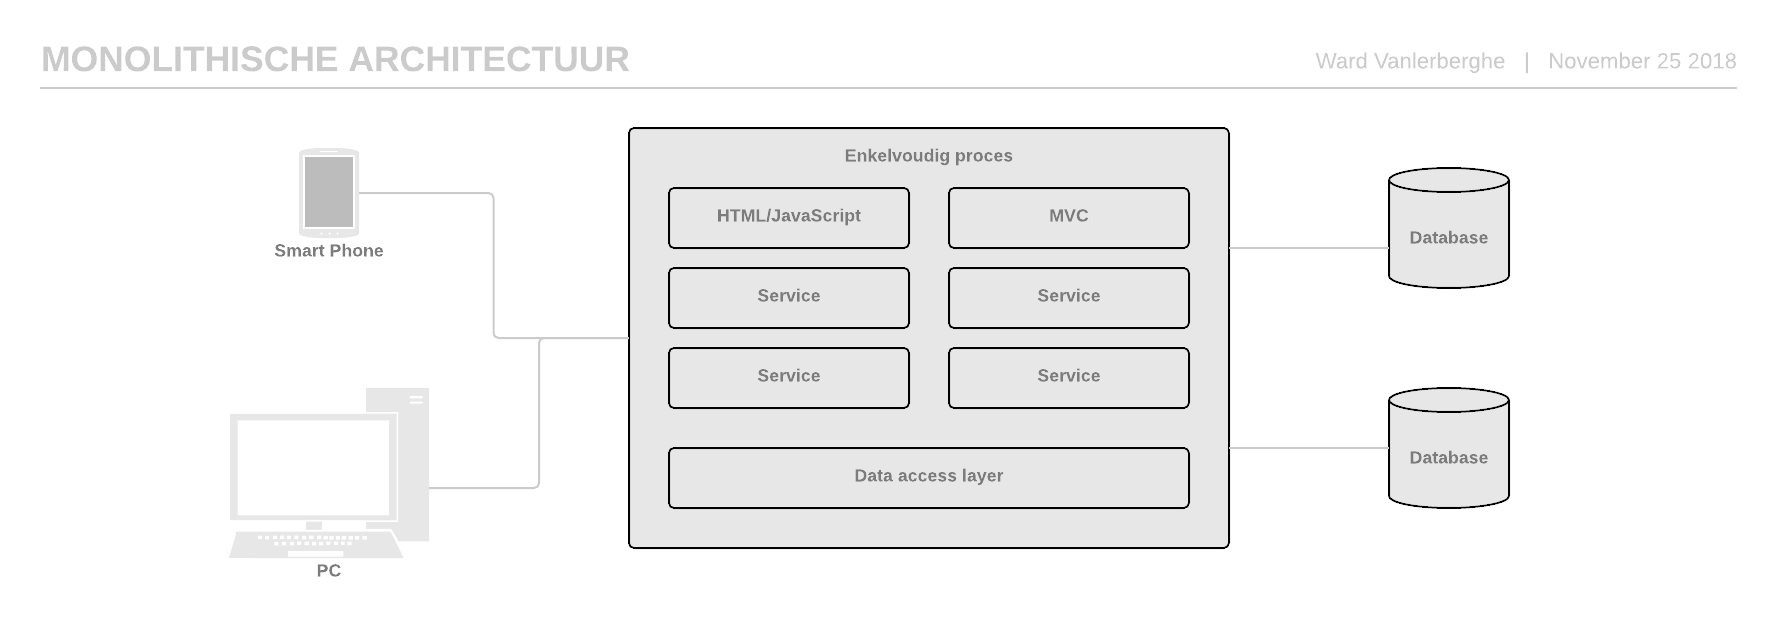
\includegraphics[width=\linewidth]{img/monolith.png}
	\caption{Weergave van een applicatie die gebruik maakt van een monolithische architectuur}
	\label{fig:monolith}
\end{figure}

Al de logica om een request af te handelen runt in één proces. Monolithische applicaties kunnen succesvol zijn. Echter meer en meer mensen voelen frustratie bij dergelijke applicaties, vooral met de toename van het deployen van applicaties naar de cloud. Elke verandering aan een kleine module van de applicatie vereist het opnieuw builden en deployen van de volledige monolithische applicatie. Na verloop van tijd word het moeilijk om een goede modulaire structuur te behouden en veranderingen die slechts aan een enkele module dienen te gebeuren worden steeds moeilijker. Indien een bepaalde module meer resources vereist dient de volledige monoliet geschaald te worden in plaats van enkel die bepaalde module. \autocite{Fowler2014}

Door deze frustraties zijn developers beginnen zoeken naar alternatieve manieren om applicaties te ontwikkelen. Dit heeft geleidt tot de microservice architectuur. Bij een microservice architectuur worden applicaties gebouwd als een verzameling van services die onafhankelijk van elkaar kunnen worden gedeployed en gescaled. Deze services communiceren doorgaans met elkaar via een \gls{REST API}. Elke service heeft een grondig afgebakende scope en volgens \textcite{Fowler2014} een eigen databank. Hoewel dit laatste niet echt een vereiste is. Echter vergt het veel discipline van de developer indien er met een gedeelde databank wordt gewerkt \autocite{Young2016}. In figuur \ref{fig:microservices} vind je een schematische voorstelling terug van een microservice architectuur.

\begin{figure}
	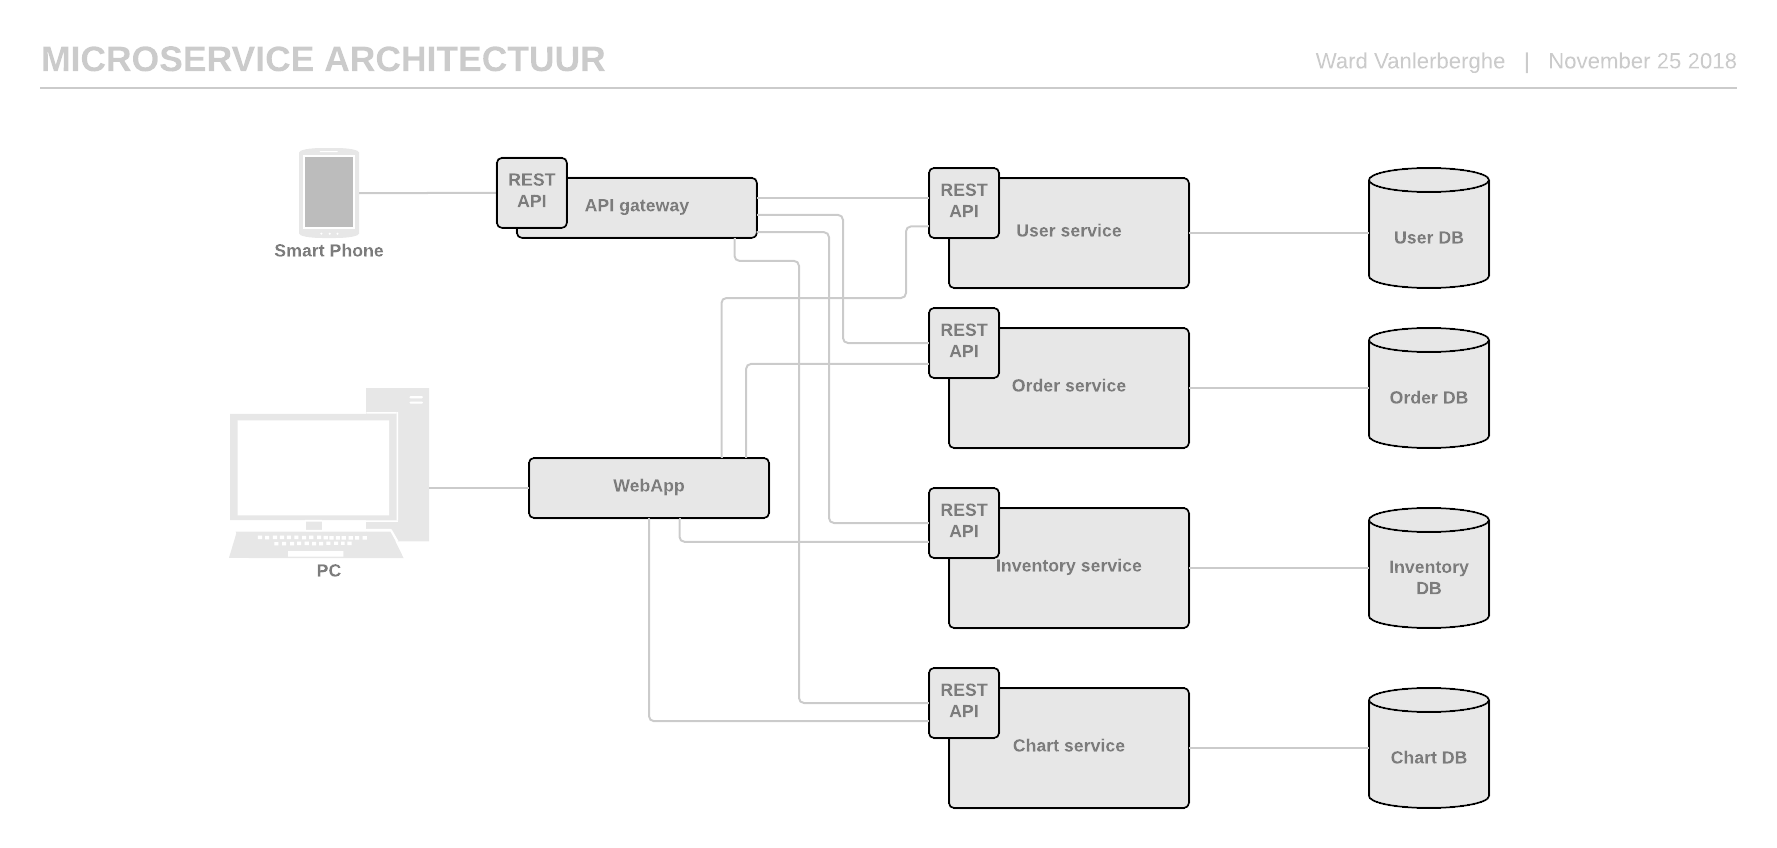
\includegraphics[width=\linewidth]{img/microservices.png}
	\caption{Weergave van een applicatie die gebruik maakt van een microservice architectuur}
	\label{fig:microservices}
\end{figure}

\section{De voordelen van een MicroService architectuur}
Zoals reeds eerder in dit hoofdstuk vermeld heeft een microservice architectuur tal van voordelen ten opzichte van een monolithische architectuur. En deze voordelen worden enkel maar groter naar gelang een applicatie groeit. Doordat de services op zo een manier van elkaar ontkoppelt zijn, is het mogelijk om voor elke service een andere programmeertaal of databanktechnologie te gebruiken. Door de modulariteit van deze architectuur kan een zeer hoge availability gegarandeerd worden, het falen van een bepaalde service hoeft niet te betekenen dat de rest van de applicatie niet bruikbaar is. Enkel de module die faalt zal tijdelijk niet toegankelijk zijn voor de eindgebruiker van de applicatie. Tevens is het veel eenvoudiger om functionaliteit aan een applicatie toe te voegen zonder de werking van de andere services (op een negatieve manier) te beïnvloeden.

Omdat de services in verschillende processen draaien wordt het ook een stuk makkelijker om \gls{DevOps} methodologieën te gaan gebruiken en de \gls{CI} en \gls{CD} principes gaan toe te passen. Deployen van nieuwe of gewijzigde functionaliteit hoeft hier geen downtime van de applicatie te betekenen.

Zoals je merkt zijn de voordelen van een microservice architectuur groot. Er zijn natuurlijk nog veel meer voordelen dan dat hier staat beschreven, maar hier nog dieper op ingaan valt buiten de scope van dit onderzoek.

In alle eerlijkheid is de microservice architectuur lang geen nieuw concept, zo  wordt beweert dat microservices hetzelfde is als \gls{SOA}, maar dan op een correcte manier uitgevoerd \autocite{Morris2014} \autocite{Young2016}. In een talk op microCon zegt \textcite{Young2016} zelfs dat het concept van microservices dateert van reeds 5 decennia geleden.

\section{De pitfalls van een MicroService architectuur}
Zoals bij vele methodieken in softwareontwikkeling, heeft ook de microservice architectuur zijn nadelen. Het is makkelijk in te beelden dat een applicatie met een groot aantal microservices al gauw zeer complex wordt.

De grote nadelen volgens \textcite{Fowler2015} en \textcite{Hummel2018} zijn:

\begin{itemize}
	\item Verschillende databanken en transactie management kunnen een pijnpunt vormen.
	\item Het testen van een applicatie met een microservice architectuur kan zeer moeizaam zijn. Dit komt omdat we voor elke microservice moeten confirmeren of deze daadwerkelijk in een healthy state is vooraleer we kunnen van start gaan met testen.
	\item Het deployen van microservices kan complex zijn. Ze kunnen coördinatie nodig hebben tussen verschillende services en extra configuratie vereisen.
	\item Het ontwikkelen van \gls{gedistribueerde systemen} kan complex zijn. Aangezien alles nu een onafhankelijke service is, moet je er voor zorgen dat elke request op een correcte manier doorheen de verschillende services propageert. Na verloop van tijd zullen complicaties ontstaan waarbij \gls{HTTP-request} onderhevig zijn aan hoge \gls{latencies}.
\end{itemize}

Voor elk van deze nadelen bestaat er natuurlijk een oplossing \autocite{Hummel2018}. In dit onderzoek gaan we met name twee tools bespreken en vergelijken om op de laatste pitfall uit bovenstaande lijst een antwoord te bieden.

\section{Distributed Tracing}
Distributed tracing is een methode om applicaties te monitoren, hoofdzakelijk applicaties die gebruik maken van de microservice architectuur. Door het instrumenteren van code ontstaat een zogenaamde trace. Deze trace geeft ons informatie over de performantie van het systeem in de vorm van spans, zie figuur \ref{fig:trace}. Bv. hoe lang een bepaalde request nodig heeft om antwoord te geven aan de caller. Een span is hierbij de metadata van een unit of work voor een bepaalde \gls{REST} call, uitvoering van een methode, databank call,...

Op deze manier kunnen we dus belangrijke informatie vergaren over de werking van het systeem. Door het analyseren van deze traces kunnen we de code van de applicatie optimaliseren en \gls{latencies} van requests verlagen.

Distributed tracing is geen nieuw concept, Google bracht in 2010 reeds de paper \begin{quotation}
	"Dapper, a Large-Scale Distributed Systems Tracing Infrastructure"
\end{quotation} uit \autocite{36356}. Waarin de auteurs de nood van distributed tracing beschrijven en hoe ze dit hebben aangepakt binnen Google. Deze paper ligt aan de basis van veel distributed tracing tools vandaag voor handen \autocite{Mace2017}.

\begin{figure}
	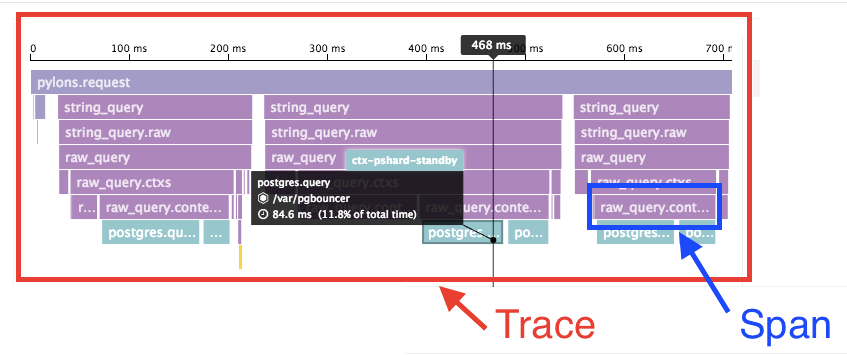
\includegraphics[width=\linewidth]{img/trace_span.png}
	\caption{Visuele weergave van een trace bestaande uit meerdere spans. Helemaal bovenaan zie je de root span, dit is de origine van de request en beschrijft de totale tijd die benodigd is om de request uit te voeren.  Onder de root span zie je de child spans. Deze beschrijven de benodigde tijd van de child requests. Het geheel van root en child spans vormt de trace. \textit{- https://datadog-docs.imgix.net/images/getting\_started/trace\_span\_image-9feba0bf.png}}
	\label{fig:trace}
\end{figure}

\section{OpenTracing}
Het grote probleem dat ontstond bij distributed tracing was dat elke tool zijn eigen implementatie van een trace had. Hierdoor was het niet makkelijk om in een lopend project van tooling te veranderen indien de tool niet langer aan de verwachtingen van het systeem voldeed. Er ontstond als het ware een \gls{vendor lock-in}.

De nood om een standaard te ontwikkelen die het mogelijk maakt om een applicatie te instrumenteren zonder vast te hangen aan een bepaalde tool was dus groot. In deze optiek werd OpenTracing\footnote{https://opentracing.io/} ontwikkeld onder de vlag van \gls{CNCF}\footnote{https://www.cncf.io/}. OpenTracing is een standaard die developers van applicaties, \gls{OSS} packages en \gls{OSS} services, toelaat om hun code te instrumenteren zonder zich aan een bepaalde tracing vendor te binden. Eerdere pogingen om een standaard te creëren voor distributed tracing focusten zich enkel op het encoderen en representatie van de trace en context data. Zowel inkomende als uitgaande. Echter is dit niet voldoende om een \gls{vendor lock-in} te vermijden \autocite{Sigelman2016}.

OpenTracing biedt verscheidene standaarden aan om dit toch te verwezenlijken \autocite{Sigelman2016}. Er is een standaard beschikbaar om spans te managen. Via simpele \gls{API}'s kan een operatie voorzien worden van een span, de span starten, stoppen of \gls{decoreren}. Verder voorziet OpenTracing een standaard, wederom met behulp van simpele \gls{API}'s, om deze spans in de vorm van een trace door te geven over de grenzen van een proces heen. Deze trace context kan ook over de grenzen van packages gepropageerd worden binnen een single proces. OpenTracing specificeert tevens een standaard voor het encoderingsformaat van de tracing context. Hierdoor kan deze context gebruikt worden door verschillende trace collectors. Enkele voorbeelden hiervan zijn Zipkin\footnote{https://openzipkin.io} en Jaeger\footnote{https://jaeger.io}.

\section{OpenCensus}
Net als OpenTracing tracht OpenCensus een antwoord te bieden op de wildgroei aan verschillende implementaties van traces. Het is een vrij nieuw initiatief dat werd opgestart door Google. De eerste release dateert van begin 2018. Het is gebaseerd op Google's interne tracing framework Census, wat al enkele jaren gebruikt wordt door Google.

Op het tijdstip van dit schrijven zijn reeds grote stappen gezet naar de verdere ontwikkeling van OpenCensus. Bij de eerste release werden slechts twee tracing collectors ondersteund, namelijk Zipkin en Google's Stackdriver\footnote{https://cloud.google.com/stackdriver/}. Door een samenwerking met Microsoft en de opensource community zijn nog geen jaar later een veel uitgebreider assortiment aan collectors beschikbaar voor OpenCensus. Momenteel worden er acht verschillende collectors ondersteund voor tracing en is er ondersteuning voor zeven verschillende programmeertalen.

Tot zover zijn de verschillen tussen OpenTracing en OpenCensus niet erg groot. Ze voorzien beiden een standaard om traces te beschrijven en te exporteren naar tracing collectors. OpenCensus biedt echter nog een extra in vergelijking met OpenTracing. Met name het ondersteunen van metrics collection. Metrics collection is het vergaren van verschillende performantie gerelateerde data. Met deze data kan dan een realtime application monitoring dashboard opgezet worden zoals bijvoorbeeld DataDog\footnote{https://www.datadoghq.com/} of Grafana\footnote{https://grafana.com/}. Zo zijn we altijd in staat om de actuele status van een applicatie te monitoren en tijdig in te grijpen.

\begin{figure}
	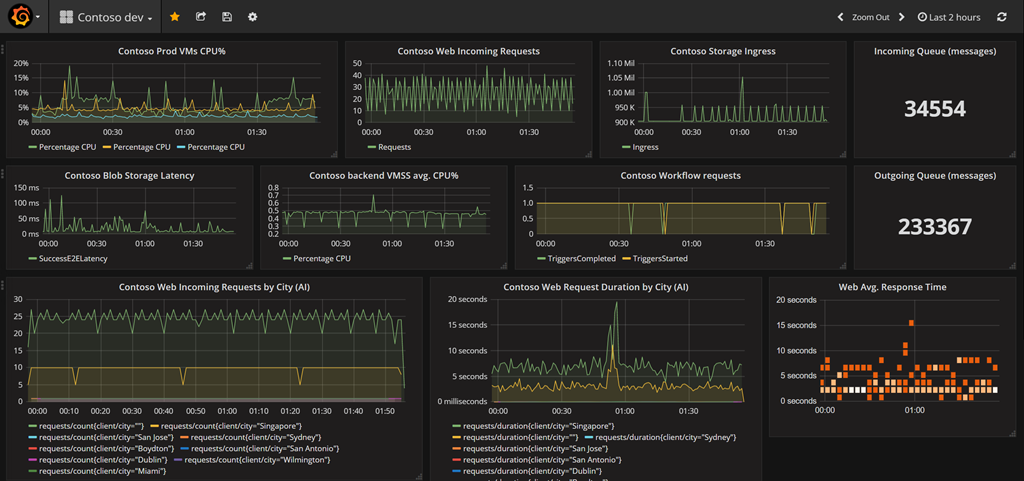
\includegraphics[width=\linewidth]{img/metrics.png}
	\caption{Een dashboard in Grafana visualiseert de vergaarde metrics via OpenCensus. \textit{- https://azurecomcdn.azureedge.net/mediahandler/acomblog/media/Default/blog/dab37ce8-46f5-4c73-9ec1-6df0e070c805.png}}
	\label{fig:metrics}
\end{figure}
%%=============================================================================
%% Methodologie
%%=============================================================================

\chapter{Methodologie}
\label{ch:methodologie}

%% TODO: Hoe ben je te werk gegaan? Verdeel je onderzoek in grote fasen, en
%% licht in elke fase toe welke stappen je gevolgd hebt. Verantwoord waarom je
%% op deze manier te werk gegaan bent. Je moet kunnen aantonen dat je de best
%% mogelijke manier toegepast hebt om een antwoord te vinden op de
%% onderzoeksvraag.




% Voeg hier je eigen hoofdstukken toe die de ``corpus'' van je bachelorproef
% vormen. De structuur en titels hangen af van je eigen onderzoek. Je kan bv.
% elke fase in je onderzoek in een apart hoofdstuk bespreken.

%\input{...}
%\input{...}
%...

%%=============================================================================
%% Conclusie
%%=============================================================================

\chapter{Conclusie}
\label{ch:conclusie}

%% TODO: Trek een duidelijke conclusie, in de vorm van een antwoord op de
%% onderzoeksvra(a)g(en). Wat was jouw bijdrage aan het onderzoeksdomein en
%% hoe biedt dit meerwaarde aan het vakgebied/doelgroep? Reflecteer kritisch
%% over het resultaat. Had je deze uitkomst verwacht? Zijn er zaken die nog
%% niet duidelijk zijn? Heeft het onderzoek geleid tot nieuwe vragen die
%% uitnodigen tot verder onderzoek?



%%=============================================================================
%% Bijlagen
%%=============================================================================

\appendix

%%---------- Onderzoeksvoorstel -----------------------------------------------

\chapter{Onderzoeksvoorstel}

Het onderwerp van deze bachelorproef is gebaseerd op een onderzoeksvoorstel dat vooraf werd beoordeeld door de promotor. Dat voorstel is opgenomen in deze bijlage.

% Verwijzing naar het bestand met de inhoud van het onderzoeksvoorstel
%---------- Inleiding ---------------------------------------------------------

\section{Introductie} % The \section*{} command stops section numbering
\label{sec:introductie}

\subsection{Context}
Meer en meer organisaties kiezen voor een microservice
architectuur bij het implementeren van nieuwe software
oplossingen. Ook bestaande monolitische applicaties
worden geleidelijk vervangen door microservice
ecosystemen. In dergelijke complexe, gedistribueerde
landschappen is het van nog groter belang om over deftige
logging en tracing te beschikken om eventuele problemen
te kunnen aanpakken.

\subsection{Nood}
Er is momenteel een wildgroei aan initiatieven die allemaal
een antwoord pogen te geven op het probleem van tracing
en metrics collectie voor gedistribueerde (microservice)
systemen.

Als Java service en solution provider is het de taak van XPLORE om
hun klanten bij te staan in een wereld waarin technologie
steeds sneller evolueert. Klanten advies kunnen geven over
cutting- en bleeding-edge technologie is één van de punten
waar hun toegevoegde waarde ligt.
In deze is het voor hen van belang een duidelijk zicht te
krijgen op welke oplossing voor distributed tracing ze in
welke context naar voor kunnen schuiven. 

\subsection{Doelstelling}
Het onderzoek bestaat uit het uitvoeren van een studie van deze 
strategie waarbij in kaart gebracht wordt wat de verschillende 
voor- en nadelen, benaderingen, hulpmiddelen, etc. zijn bij een 
polycloud aanpak.

%---------- Stand van zaken ---------------------------------------------------

\section{State-of-the-art}
\label{sec:state-of-the-art}

\subsection{Distributed tracing}
Distributed tracing is een techniek die wordt toegepast in het veld van gedistribueerde software systemen, ook wel microservices genoemd, die het toelaat om inzicht te krijgen over de interne samenwerking tussen deze verschillende services. Het laat toe om na te gaan waar in het systeem (lees: " in welke microservice") er iets fout loopt of waar zich een bottleneck bevindt. OpenTracing is hierbij zowat de de-facto standaard geworden voor dergelijke oplossingen.

Het instrumenteren van systemen om distributed tracing te ondersteunen was tot voor kort nog een werkintensieve en complexe opdracht. De OpenTracing standaard bracht hier verandering in en zorgt ervoor dat het instrumenteren van applicaties voor gedistribueerde tracing met een minimum aan inspanning kan verwezenlijkt worden. 

Sinds Oktober 2016 richt OpenTracing, onder begeleiding van Cloud Native Computing Foundation (CNCF), er zich op om een open, verkoperneutrale standaard voor gedistribueerde systeem instrumentatie te zijn. Het biedt developers een manier om requests te traceren van het begin tot het einde, en dit van simpele gedistribueerde systemen met slechts enkele services tot zeer complexe gedistribueerde systemen met honderden services verdeeld over verschillende systemen en zelfs verschillende fysieke locaties.

In OpenTracing vertelt elke trace het verhaal van een transactie of een workflow die zich propageert doorheen het gedistribueerde systeem. Een trace maakt gebruik van een gerichte graaf die geen cycles bevat, elke knoop in de graaf stelt dan een stap voor in het proces met bijhorende metrics over deze stap. \autocite{Arbezzano2017}

\subsection{Tracing \& metrics systemen}
Zoals in de introductie reeds vermeld is er momenteel een wildgroei aan initiatieven die een antwoord pogen te geven op het probleem van tracing en metrics collectie voor gedistribueerde systemen. Enkele voorbeelden hiervan zijn Zipkin (Twitter) en Jaeger (CNCF), die beiden de OpenTracing standaard supporten. Dergelijke systemen bieden een UI aan waarin je op een snelle en overzichtelijke manier traces met bijhorende metrics kan visualiseren om problemen in het geinstrumenteerde systeem te kunnen opsporen. Doordat dergelijke systemen de OpenTracing standaard supporten zou het op zich gemakkelijk moeten zijn om een dergelijk systeem door een nieuw systeem te vervangen, of zelfs simultaan naast elkaar te laten draaien.

% Voor literatuurverwijzingen zijn er twee belangrijke commando's:
% \autocite{KEY} => (Auteur, jaartal) Gebruik dit als de naam van de auteur
%   geen onderdeel is van de zin.
% \textcite{KEY} => Auteur (jaartal)  Gebruik dit als de auteursnaam wel een
%   functie heeft in de zin (bv. ``Uit onderzoek door Doll & Hill (1954) bleek
%   ...'')

%---------- Methodologie ------------------------------------------------------
\section{Methodologie}
\label{sec:methodologie}

In eerste instantie zal er een simplistisch gedistribueerd systeem ontwikkeld worden, dit systeem moet dienen als System Under Test (SUT) en moet een real life gedistribueerd systeem met bottlenecks simuleren. Dit kan op een eenvoudige manier gebeuren door een thread voor een bepaalde tijd te laten wachten. De verschillende services zullen elk in hun eigen Docker/Kubernetes container gedeployed worden. De code van deze services zal geïnstrumenteerd worden met behulp van de OpenTracing standaard.

Eenmaal deze testomgeving is opgesteld kunnen we op een gemakkelijk manier de verschillende systemen voor de tracing en metrics visualisatie gaan vergelijken. Aangezien de simpliciteit van het SUT kunnen we ook gemakkelijk nagaan of de verschillende systemen consistente data visualiseren.

Er zal vooral gekeken worden naar volgende punten:
\begin{itemize}
	\item Correctheid traces en metrics
	\item Moeilijkheidsgraad in het instrumenteren van de code
	\item Moeilijkheidsgraad opzetten van het systeem
	\item Grote community
\end{itemize}

In tweede instantie zal met de gegenereerde data een bevraging worden uitgevoerd bij developers. Met behulp van de gegenereerde data zal voor beide systemen gevraagd worden om zo snel mogelijk de bottleneck in het systeem te vinden. Aan de hand van de snelheid waarmee een bottleneck kan worden gevonden door een developer zal een conclusie trachten gemaakt te worden met welk systeem het meest vlot gewerkt kan worden.

%---------- Verwachte resultaten ----------------------------------------------
\section{Verwachte resultaten}
\label{sec:verwachte_resultaten}

Aangezien de OpenTrace standaard en bijhorende systemen relatief nieuw zijn, is het moeilijk om hier reeds een verwacht resultaat neer te zetten. Verwacht word echter wel dat Jaeger gemakkelijker te instrumenteren zal zijn, aangezien dit systeem werd ontwikkeld door CNCF, die ook het OpenTrace project begeleid. De vergelijking over hoe vlot de metrics uit de systemen zijn te halen is echter moeilijker te concluderen. Veel zal hier afhangen van hoe goed de ontwerpers aan de flow van de systemen heeft gedacht.

%---------- Verwachte conclusies ----------------------------------------------
\section{Verwachte conclusies}
\label{sec:verwachte_conclusies}

Aangezien er met een bepaalde standaard gewerkt wordt, namelijk de OpenTracing standaard, worden er geen grote, of misschien zelfs geen, verschillen verwacht in de instrumentatie van de code. Er wordt wel verwacht dat Jaeger gemakkelijker integreerbaar zal zijn in een gedistribueerde systemen die reeds in containers draaien. Dit vooral omdat het systeem ontwikkeld is door CNCF en dus beter in het ecosysteem van Cloud en Microservices zal integreren.



%%---------- Andere bijlagen --------------------------------------------------
% TODO: Voeg hier eventuele andere bijlagen toe
%\input{...}

%%---------- Referentielijst --------------------------------------------------

\printbibliography[heading=bibintoc]
%\addcontentsline{toc}{chapter}{\textcolor{maincolor}{\IfLanguageName{dutch}{Bibliografie}{Bibliography}}}

\end{document}
